 \documentclass{report}

\usepackage{fancyhdr}
\usepackage{parskip}
\usepackage{amsmath}
\usepackage[linguistics]{forest}
\usepackage[shortlabels]{enumitem}
\usepackage{caption}
\usepackage{tikz}
\usetikzlibrary{automata, positioning, arrows}
\tikzset{
->, % makes the edges directed
>=stealth, % makes the arrow heads bold
node distance=2cm, % specifies the minimum distance between two nodes. Change if necessary.
every state/.style={thick, fill=gray!10}, % sets the properties for each ’state’ node
initial text=$ $, % sets the text that appears on the start arrow
}

\newcommand\Mydiv[2]{%
$\strut#1$\kern.25em\smash{\raise.3ex\hbox{$\big)$}}$\mkern-8mu
        \overline{\enspace\strut#2}$}


\pagestyle{fancy}
\fancyhf{Aaron Pierce}
\rhead{\today}
% DON'T FORGET TO CHANGE THIS vvvvvvvvvvv
\lhead{CS-3823 Homework 3}
% DON'T FORGET TO CHANGE THIS ^^^^^^^^^^^
\fancyfoot{}


\begin{document}
    \section*{Problem 1}
    Find all strings in $L((a+bb)^*))$ of length 5
    \begin{itemize}
        \item zero instances of bb
        \begin{enumerate}
            \item aaaaa
        \end{enumerate}

        \item one instance of bb
        \begin{enumerate}
            \item[2.] aaabb
            \item[3.] aabba
            \item[4.] abbaa
            \item[5.] bbaaa
        \end{enumerate}

        \item two instances of bb
        \begin{enumerate}
            \item[6.] bbbba
            \item[7.] bbabb
            \item[8.] abbbb
        \end{enumerate}
    \end{itemize}

    \section*{Problem 3}
    Find an NFA that accepts the language $L(aa^* (ab + b))$.

    \begin{figure}[ht] % ’ht’ tells LaTeX to place the figure ’here’ or at the top of the page
        \centering % centers the figure
        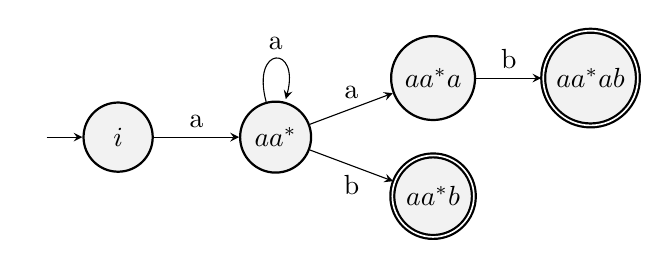
\begin{tikzpicture}

            \node[state, initial] (i) {$i$};
            \node[state, right of=i] (a) {$aa^*$};
            \node[state, right of=a, yshift=0.75cm] (na) {${aa^*a}$};
            \node[state, accepting, right of=a, yshift=-0.75cm] (nb) {${aa^*b}$};
            \node[state, accepting, right of=na] (nab) {${aa^*ab}$};
            \draw   (i) edge[above] node{a} (a)
                    (a) edge[loop above] node{a} (a)
                    (a) edge[above] node{a} (na)
                    (a) edge[below] node{b} (nb)
                    (na) edge[above] node{b} (nab);
        \end{tikzpicture}
        \caption{Accepts $L(aa^* (ab + b))$}
        \label{fig:p3}
    \end{figure}


    \section*{Problem 7}
    Find a regular expression for the set $\left\{a^nb^m : n \geq 3, m \text{ is odd}\right\}$.

    \textbf{Answer:} $(aaaa^*)(b(bb)^*)$
\\
    \section*{Problem 18}
    Find a regular expression for:
    \begin{gather*}
        L = \left\{ w \in \left\{ 0, 1\right\}^* \text{ : } w \text{ has exactly one pair of consecutive zeroes} \right\}
    \end{gather*}
    \textbf{Answer: } $\left(0 + \lambda\right)\left(\left(1 + 101\right)^*\right) \left(00\right) \left(\left(1 + 101\right)^*\right) \left(0 + \lambda\right)$

    \section*{Problem 5}
    Give an nfa that accepts the language 
    $L\left( \left(a+b\right)^* b \left(a+bb\right)^* \right)$

    \begin{figure}[ht] % ’ht’ tells LaTeX to place the figure ’here’ or at the top of the page
        \centering % centers the figure
        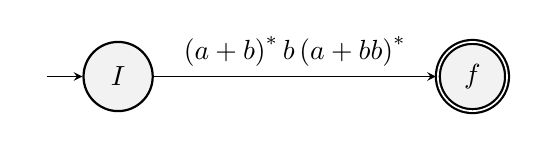
\begin{tikzpicture}

            \node[state, initial, xshift=-2.5cm] (i) {$I$};
            \node[state, accepting, right of=i, xshift=2.5cm] (f) {$f$};
            \draw   (i) edge[above] node{$\left(a+b\right)^* b \left(a+bb\right)^*$} (f);
        \end{tikzpicture}
        \caption*{Step 1, make a trivial NFA}
        \label{fig:p5s1}
    \end{figure}

    \begin{figure}[ht] % ’ht’ tells LaTeX to place the figure ’here’ or at the top of the page
        \centering % centers the figure
        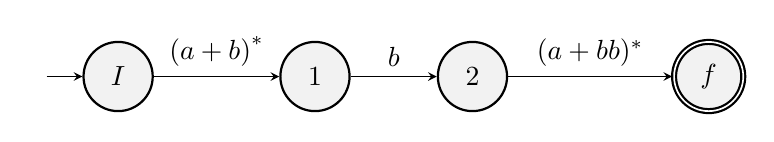
\begin{tikzpicture}

            \node[state, initial, xshift=-1cm] (i) {$I$};
            \node[state, right of=i, xshift=0.5cm] (abstar) {1};
            \node[state, right of=abstar] (b) {2};
            \node[state, accepting, right of=b, xshift=1cm] (f) {$f$};
            \draw   (i) edge[above] node{$\left(a+b\right)^*$} (abstar);
            \draw   (abstar) edge[above] node{$b$} (b);
            \draw   (b) edge[above] node{$(a+bb)^*$} (f);
        \end{tikzpicture}
        \caption*{Step 2, split off the concats}
        \label{fig:p5s2}
    \end{figure}

    \begin{figure}[ht] % ’ht’ tells LaTeX to place the figure ’here’ or at the top of the page
        \centering % centers the figure
        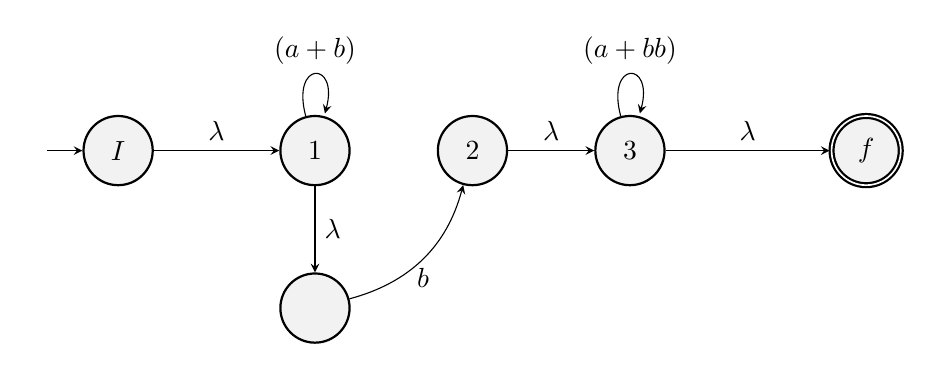
\begin{tikzpicture}

            \node[state, initial, xshift=-1cm] (i) {$I$};
            \node[state, right of=i, xshift=0.5cm] (abstar) {1};
            \node[state, right of=i, xshift=0.5cm, yshift=-2cm] (pas) {};
            \node[state, right of=abstar] (b) {2};
            \node[state, right of=b] (apb) {3};
            \node[state, accepting, right of=apb, xshift=1cm] (f) {$f$};
            \draw   (i) edge[above] node{$\lambda$} (abstar);
            \draw   (abstar) edge[loop above] node{$\left(a+b\right)$} (abstar);
            \draw   (abstar) edge[right] node{$\lambda$} (pas);
            \draw   (pas) edge[below, bend right] node{$b$} (b);
            \draw   (b) edge[above] node{$\lambda$} (apb);
            \draw   (apb) edge[loop above] node{$\left(a+bb\right)$} (apb);
            \draw   (apb) edge[above] node{$\lambda$} (f);
        \end{tikzpicture}
        \caption*{Step 3, expand kleene stars}
        \label{fig:p5s3}
    \end{figure}

    \begin{figure}[ht] % ’ht’ tells LaTeX to place the figure ’here’ or at the top of the page
        \centering % centers the figure
        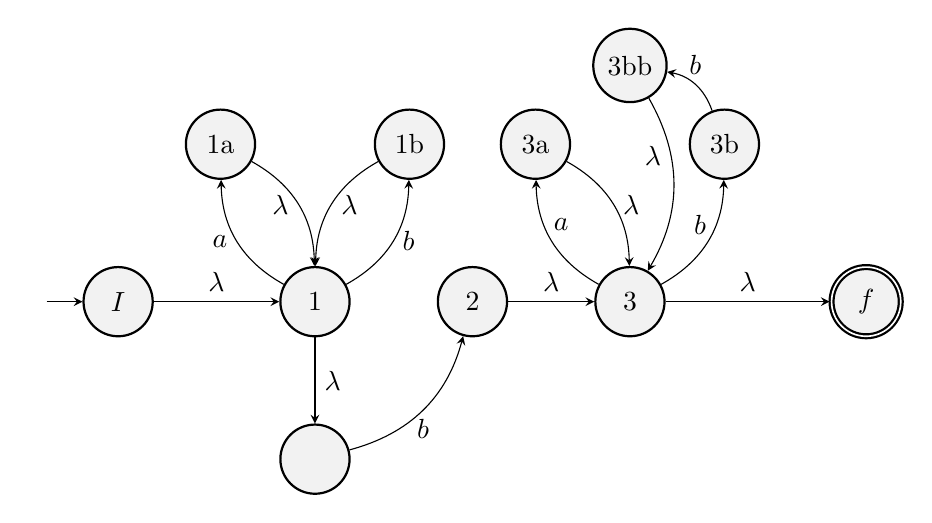
\begin{tikzpicture}

            \node[state, initial, xshift=-1cm] (i) {$I$};

            \node[state, right of=i, xshift=0.5cm] (abstar) {1};
            \node[state, left of=abstar, yshift=2cm, xshift=0.8cm] (abstara) {1a};
            \node[state, right of=abstar, yshift=2cm, xshift=-0.8cm] (abstarb) {1b};
            \node[state, right of=i, xshift=0.5cm, yshift=-2cm] (pas) {};
            
            \node[state, right of=abstar] (b) {2};
            
            \node[state, right of=b] (apb) {3};
            \node[state, left of=apb, yshift=2cm, xshift=0.8cm] (apba) {3a};
            \node[state, right of=apb, yshift=2cm, xshift=-0.8cm] (apbb) {3b};
            \node[state, right of=b, yshift=3cm] (apbbb) {3bb};
            
            \node[state, accepting, right of=apb, xshift=1cm] (f) {$f$};
            \draw   (i) edge[above] node{$\lambda$} (abstar);
            \draw   (abstar) edge[left, bend left] node{$a$} (abstara);
            \draw   (abstara) edge[left, bend left] node{$\lambda$} (abstar);
            \draw   (abstar) edge[right, bend right] node{$b$} (abstarb);
            \draw   (abstarb) edge[right, bend right] node{$\lambda$} (abstar);
            \draw   (abstar) edge[right] node{$\lambda$} (pas);
            \draw   (pas) edge[below, bend right] node{$b$} (b);
            \draw   (b) edge[above] node{$\lambda$} (apb);

            \draw   (apb) edge[right, bend left] node[pos=0.65]{$a$} (apba);
            \draw   (apba) edge[right, bend left] node{$\lambda$} (apb);
            \draw   (apb) edge[left, bend right] node[pos=0.65]{$b$} (apbb);
            \draw   (apbb) edge[above, bend right] node{$b$} (apbbb);
            \draw   (apbbb) edge[left, bend left] node[pos=0.33]{$\lambda$} (apb);
            
            \draw   (apb) edge[above] node{$\lambda$} (f);
        \end{tikzpicture}
        \caption*{Step 4, break off unions.\\ \\
        All labels are now single symbols, so the NFA is complete.\\
        Leaving node 1 we have $\left(a+b\right)^*$.\\
        Leaving node 2 we have $\left(a+b\right)^* b$\\
        And leaving node 3 we finish with $\left(a+b\right)^* b \left(a+bb\right)^*$
        }
        \label{fig:p5s4}
    \end{figure}

    \pagebreak
    \section*{Problem 7(b)}
    Find a DFA to accept $L = L\left( ab^* a^*\right) \cap L\left( b^*ab \right)$

    \begin{figure}[ht] % ’ht’ tells LaTeX to place the figure ’here’ or at the top of the page
        \centering % centers the figure
        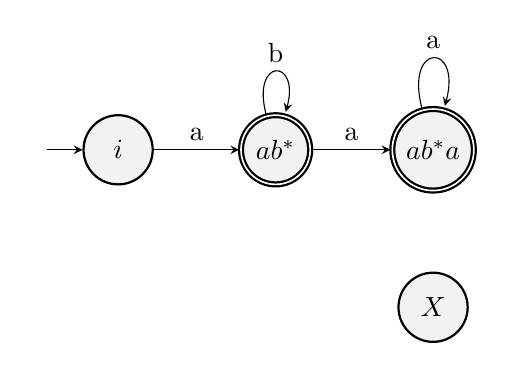
\begin{tikzpicture}

            \node[state, initial] (i) {$i$};
            \node[state, right of=i, accepting] (a) {$ab^*$};
            \node[state, right of=a, accepting] (aba) {$ab^*a$};
            \node[state, right of=a, yshift=-2cm] (x) {$X$};
            % \node[state, right of=a, yshift=0.75cm] (na) {${aa^*a}$};
            % \node[state, accepting, right of=a, yshift=-0.75cm] (nb) {${aa^*b}$};
            % \node[state, accepting, right of=na] (nab) {${aa^*ab}$};
            \draw   (i) edge[above] node{a} (a)
                    (a) edge[loop above] node{b} (a)
                    (a) edge[above] node{a} (aba)
                    (aba) edge[loop above] node{a} (aba)
                    ;
        \end{tikzpicture}
        \caption*{Step 1, design DFA for $L\left( ab^* a^*\right)$}
        \label{fig:p7bs1}
    \end{figure}
\end{document}